\newpage
\section{Attori del sistema}
\vspace{-8mm}
\begin{figure}[!h]
    \centering
    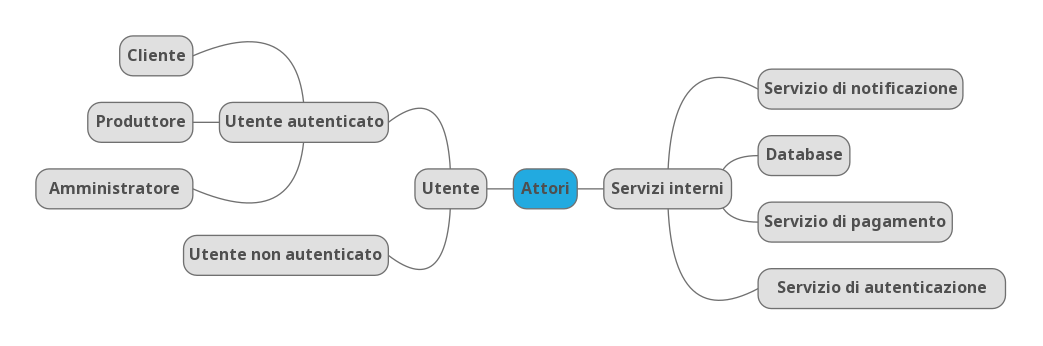
\includegraphics[width=1\linewidth]{Deliverables/first-deliverable/img/mappa_attori.png}
    \label{fig:mindmap}
\end{figure}

\vspace{-10mm}


\begin{attori}
     \item \textbf{Utente}: Generico utente che ha la possibilità di visualizzare la lista delle aziende produttrici, la loro valutazione e le relative recensioni, di consultare il catalogo dei prodotti in vendita, di ricercare aziende e prodotti tramite parole chiave e di visualizzare le ultime notizie ed aggiornamenti riguardanti il mercato contadino di Trento, in aggiunta ad orari e luoghi di svolgimento dello stesso.
     \begin{enumerate}
         \item \textbf{Utente non autenticato}: Interazioni limitate come Utente. Ha inoltre la possibilità di registrarsi (Sign up), di autenticarsi (Log in) tramite email e password o di recuperare quest'ultima.
         
         \item \textbf{Utente autenticato}: Utente che ha fatto l'accesso al sistema e che ha in aggiunta la possibilità di accedere ad un'area privata dove può modificare i propri dati.
     
         \begin{enumerate}
             \item \textbf{Cliente}: Dispone di tutte le interazioni possibili per l'utente autenticato. In aggiunta può prenotare i prodotti in vendita, richiedere la consegna a domicilio, e scegliere fra due opzioni di pagamento: online o presso il punto vendita. L'area privata consentirà di visualizzare le prenotazioni effettuate e i dettagli relativi all'account. Ha inoltre la possibilità di visualizzare e lasciare recensioni ai produttori. 
             
             \item \textbf{Produttore}: Dispone di tutte le interazioni possibili per l'utente autenticato. In aggiunta ha la possibilità di gestire i prodotti in vendita, inserendo i prodotti nuovi con relativi dettagli, e rimuovendo quelli esauriti. Può inoltre inserire offerte e promozioni per i clienti. L'area privata consentirà di monitorare sia gli ordini attivi che quelli completati, anche mediante l'utilizzo di dashborad interattive e la generazione di report relativi alle vendite e incassi.
             
              \item \textbf{Amministratore}: Ha la possibilità di visualizzare, controllare e modificare tutti gli account registrati in modo da risolvere eventuali problematiche. Monitora l’andamento della piattaforma, supervisiona il corretto utilizzo della stessa e modera le recensioni e feedback degli utenti.
              Ha infine il controllo completo sulla gestione degli avvisi pubblici: può pubblicare aggiornamenti su spostamenti del mercato, chiusure straordinarie ed eventi speciali.
 
         \end{enumerate}
     \end{enumerate}
 
     \item \textbf{Servizi Interni}
     \begin{enumerate}
         \item \textbf{Database}: Memorizza dati su utenti, venditori e prodotti, gestisce ordini, pagamenti e recensioni. Conserva inoltre dati su disponibilità e stagionalità dei prodotti e archivia statistiche e report di vendita.
         \item \textbf{Servizio di Pagamento}: Gestisce le transazioni online in sicurezza e supporta pagamenti flessibili (anticipati o alla consegna).
         \item \textbf{Servizio di Autenticazioane}: Gestisce la registrazione e il login degli utenti. Supporta autenticazione tramite email e password. Controlla permessi e ruoli (cliente, venditore e amministratore) e garantisce la sicurezza dei dati.
         \item \textbf{Servizio di Notificazione}: Invia conferme d’ordine ai clienti, ricorda le scadenze per il ritiro degli ordini e notifica i venditori sugli ordini ricevuti. 
     \end{enumerate}
 \end{attori}

\newpage